\documentclass{pjatk}

\usepackage{tocloft}
\usepackage{hyperref}
\usepackage[english,polish]{babel}
\usepackage{tikz-uml}
\usepackage[acronym, toc]{glossaries}

\addbibresource{attachments/bibliography.bip}

\makeglossaries
%! Author = Mateusz Budzisz
%! Date = 08/11/2023

\newglossaryentry{pwa}{name={Progressive Web App},
description={Progressive Web App (PWA) to progresywna aplikacja internetowa uruchamiana tak jak zwykła strona internetowa,
 ale umożliwiająca stworzenie wrażenia działania jak natywna aplikacja mobilna lub aplikacja desktopowa. }
}
\newglossaryentry{aws}{name={Amazon Web Services},
description={Amazon Web Services (AWS) – pakiet usług chmurowych oferowanych przez Amazon},
}
\newglossaryentry{gcp}{name={Google Cloud Platform},
description={Oferowany przez Google zestaw usług chmurowych, obejmuje szereg modułowych usług chmurowych, w tym przetwarzanie danych, przechowywanie danych, analitykę danych oraz uczenie maszynowe, a także zestaw narzędzi zarządzania.}
}
\newglossaryentry{azure}{ name={Azure},
description={Microsoft Azure to platforma chmurowa firmy Microsoft stworzona w modelu PaaS (Platform as a Service)}
}
\newglossaryentry{osm}{name={Open Street Map},
description={OpenStreetMap (OSM) – projekt społeczności internetowej mający na celu stworzenie darmowej, swobodnie dostępnej mapy całej kuli ziemskiej.}}
\newglossaryentry{lsp}{name={Language Service Protocol},
description={Protokół Language Server Protocol (LSP) to otwarty protokół oparty na JSON-RPC, stosowany pomiędzy edytorami kodu źródłowego lub zintegrowanymi środowiskami programistycznymi (IDE) a serwerami, które dostarczają "narzędzia inteligencji językowej": specyficzne dla języków programowania funkcje, takie jak uzupełnianie kodu, podświetlanie składni oraz oznaczanie ostrzeżeń i błędów, a także rutyny refaktoryzacji.}
}
\newglossaryentry{osw}{
name={Open Weather Map},
description={Open Weather Ma} 
}
\newglossaryentry{http}{name={Hyper Text Transfer Protocol},
description={ Hyper Text Transfer Protocol protokół stworzony przez Tima Bernersa-Lee na potrzeby komunikacji między klientem a serwerem w sieci WWW (ang. World Wide Web).}
}

\newglossaryentry{drag-n-drop}
{
    name={Drag and drop},
    description={Technologia umożliwiająca interfejsom użytkownika w przeglądarkach internetowych korzystanie z funkcji przeciągania i upuszczania elementów. Użytkownik może wybrać elementy do przeciągania za pomocą myszy, przeciągnąć te elementy do elementu docelowego i upuścić je, zwalniając przycisk myszy. Podczas operacji przeciągania półprzezroczysta reprezentacja przeciąganych elementów podąża za wskaźnikiem myszy.}
}

\newglossaryentry{on-demand}
{
    name={On-demand},
    description={Rodzaj oprogramowania charakteryzującego się dynamicznym czasem pracy, uruchamiane na rządanie, gdy poda wynik program kończy pracę zamiast oczekiwać następnego zapytania}
}

\newglossaryentry{refactoring}
{
    name={Refactoring},
    description={Znaczna zmiana konstrukcji programu mająca na celu usprawnienie oprogramowania bądź dostosowanie go do nowych wymogów}
}

\newglossaryentry{ui}
{
    name={UI},
    description={Interfejs użytkownika}
}

\newglossaryentry{frontend}
{
    name={Frontend},
    description={Oprogramowanie składające się z UI z którym docelowy użytkownik będzę wchodził w interakcję}
}

\newglossaryentry{backend}
{
    name={Backend},
    description={Oprogramowanie pozbawione UI z którym docelowy użytkownik będzę wchodził w interakcję, potrzebne do prawidłowej pracy Frontendu}
}

\newglossaryentry{job}
{
    name={Job},
    description={Oprogramowanie, które ma z góry określony cel, po jego uruchomieniu natychmiast zaczyna je wykonywać, nie wchodzi w interakcje z użytkownikiem docelowym, po zakończeniu kończy swoje życie}
}


\newglossaryentry{rendering}
{
    name={Wyrenderowanie},
    description={Stworzenie UI z postaci kodu do postaci konsumowalnej przez użytkownika docelowego}
}

\newglossaryentry{hello-world}
{
    name={Hello world},
    description={Minimalny reprezentatywny program w danej technologii}
}

\newglossaryentry{hermetyzacja}
{
    name={Hermetyzacja},
    description={Hermetyzacja opgorgramowania określa dobrą praktykę programistyczną polegającą na izolacji komponentów w aplikacji tak aby o sobie nie wiedziały gdy nie muszą o sobie wiedzieć}
}

\newglossaryentry{infra-as-code}
{
    name={Infrastructure as a code},
    description={Sposób opisania architektury systemu poprzez napisanie programu tworzącego docelową architekturę przy pomocy abstrakcji dostarczonych przez dostawcę mocy obliczeniowej}
}

\newglossaryentry{on-prem}
{
    name={On-premise},
    description={Oprogramowanie hostowane na samodzielnie zarządzanej infrastrukturze}
}

\newglossaryentry{virt}
{
    name={Wirtualizacja},
    description={Podział serwera na maszyny o mniejszej mocy obliczeniowej, aby umożliwić podział podzespołów pomiędzy klientów tak, aby nic o sobie nawzajem nie wiedzieli}
}

\newglossaryentry{arm}
{
    name={Architektura ARM},
    description={Architektura silnej ręki lol}
}
\newglossaryentry{poidef}
{
    name={POI},
    description={Point of interest (w skrócie POI) to punkt w przestrzeni, najczęściej na powierzchni Ziemi.}
}
\newglossaryentry{openlayers}
{
    name={Openlayers},
    description={OpenLayers to biblioteka napisana w języku JavaScript, ułatwiająca dodawanie dynamicznych map na stronach internetowych.}
}
\newglossaryentry{reflink}
{
    name={Reflink},
    description={Reflink to specjalny link, który zawiera unikalny kod identyfikacyjny, pozwalający na monitorowanie ruchu i przekierowań z innych źródeł.}
}
\newglossaryentry{sla}
{
    name={SLA},
    description={Service Level Agreement, SLA (umowa o gwarantowanym poziomie świadczenia usług) to umowa utrzymania i systematycznego poprawiania ustalonego między usługodawcą a usługobiorcą poziomu jakości usług poprzez stały cykl obejmując: uzgodnienia,
    monitorowanie usługi, raportowanie, przegląd osiąganych wyników.}
}
\newglossaryentry{sws}
{
    name={SWS},
    description={Specyfikacja Wymagań Systemowych }
}
\newglossaryentry{moscow}
{
    name={MoSCoW},
    description={Metoda MoSCoW to technika priorytetyzacji wykorzystywana w analizie biznesowej i przy tworzeniu oprogramowania w celu osiągnięcia wspólnego zrozumienia pomiędzy interesariuszami co do znaczenia, jakie ma dla nich dostarczenie każdego z wymagań. Inne nazwy metody to priorytetyzacja MoSCoW lub analiza MoSCoW.}
}
\newglossaryentry{CRUD}
{
    name={CRUD},
    description={CRUD (od angielskiego create, read, update, delete, tłumaczenie utwórz, odczytaj, aktualizuj, usuń) – cztery podstawowe funkcje w aplikacjach korzystających z bazy danych, które umożliwiają zarządzanie nią.}
}
\newglossaryentry{stadiamaps}
{
    name={Stadia Maps},
    description={Stadia Maps oferuje komercyjne interfejsy API do mapowania i wyznaczania tras, głównie oparte na OpenStreetMap.}
}

\newglossaryentry{mevo}
{
    name={Mevo},
    description={Mevo to system bezobsługowych wypożyczalni rowerów miejskich.}
}
\newglossaryentry{scraping}
{
    name={Web scraping},
    description={Data scraping to technika ekstrakcji danych z witryn internetowych.}
}
\newglossaryentry{lighthouse}
{
    name={Lighthouse},
description={Lighthouse to narzędzie open-source stworzone przez Google do automatycznego audytu stron internetowych. Analizuje wydajność, dostępność, zgodność z progresywnymi aplikacjami webowymi (PWA), SEO i najlepszymi praktykami. Wyniki audytów pomagają poprawić jakość i funkcjonalność stron internetowych. Narzędzie można uruchomić z poziomu Chrome DevTools, jako rozszerzenie Chrome lub z wiersza poleceń.}
}
\newglossaryentry{openmeteo}
{
    name={OpenMeteo},
description={OpenMeteo to darmowa, otwarta usługa dostarczająca prognozy pogody poprzez interfejs API. Oferuje precyzyjne prognozy dla różnych lokalizacji na świecie, umożliwiając integrację z aplikacjami i serwisami internetowymi.}
}


\studfield{Informatyka}
\studtype{Zaoczne}
\title{Planer Mapy Miejskiej}
\engtitle{City Map Planner}
\acronym{City Planner}
\titledate{2023-10-14}
\supervisor{prof. dr hab. Marek A. Bednarczyk}
\author{Mateusz Budzisz}{s24048}{Aplikacje Internetowe}{Zaoczny}
\author{Wiktor Rostkowski}{s23141}{Aplikacje Internetowe}{Zaoczny}
\author{Sebastian Kreft}{s23133}{Aplikacje Internetowe}{Zaoczny}
\author{Damian Kreft}{s23447}{Aplikacje Internetowe}{Zaoczny}
\consultant{--- brak ---} % Koniecznie trzeba podać brak, albo wpisać konsultantów tak jak przy autorach
\projectgoals{Stworzenie interaktywnej mapy miejskiej do planowania zwiedzania atrakcji turstycznych z wkykorzystaniem dynamicznych danych}
\productsandservices{Aplikacja progresywana}
\mainfunctionalities{Planowanie trasy}
\successmeasure{Wdrożenie rozwiązania jako oficjalnego rozwiązania miejskiego}
\projlimitations{Brak budżetu}
\date{\today}
\nabstract{
	Praca zakłada utworzenie interaktywnej mapy z punktami zainteresowań na podstawie listy atrakcji turystycznych wyróżnionych przez urząd miejski,
	umożliwiającej kompleksowe zaplanowanie optymalnej trasy zwiedzania z uwzględnieniem środków komunikacji miejskiej,
	godzin otwarcia atrakcji turystycznych oraz warunków pogodowych.
}

\graphicspath {{attachments/}}

\begin{document}

	% PJATK Template begin
	\maketitle
	\makeprojectcard
	\makedeclaration
	% PJATK Template End

	\tableofcontents
	\clearpage
	\include{chapters/przykłady-latex}
	%! Author = Wiktor Rostkowski
%! Date = 29/04/2024

%! Author = Wiktor Rostkowski, Mateusz Budzisz
%! Date = 29.10.2023

\chapter{Wstęp}
\label{ch:wstep}

W miastach, które oferują wiele atrakcji turystycznych oraz posiadają rozbudowane~i~złożone systemy transportu publicznego, tworzenie optymalnego planu zwiedzania może~być~skomplikowane~i~czasochłonne.
Konieczność uwzględnienia godzin otwarcia poszczególnych miejsc, dostępności różnych środków transportu oraz efektywnego wykorzystania czasu sprawia,~że~planowanie wycieczki wymaga dużej precyzji~i~uwagi.
Co więcej, uwzględnienie indywidualnych preferencji turystów, takich~jak~zainteresowania, tempo zwiedzania~czy~potrzeba przerw~na~odpoczynek, jeszcze bardziej zwiększa stopień trudności tego zadania.

Zespół projektowy wcześniej napotkał dokładnie~ten~problem,~co~doprowadziło~do~powstania pomysłu~na~stworzenie nowatorskiej aplikacji.
Aplikacja~ta~składa~się~z interaktywnej mapy, która prezentuje różnorodne atrakcje turystyczne~w~danym mieście, oraz kalendarza~w~stylu \gls{drag-n-drop}, umożliwiającego łatwe planowanie dnia.
Aplikacja uwzględnia dane~w~czasie rzeczywistym, takie~jak~prognoza pogody, aktualne informacje~o~komunikacji miejskiej oraz godziny otwarcia poszczególnych atrakcji.
Ponadto aplikacja oferuje interaktywny widok, który automatycznie generuje optymalną trasę zwiedzania zgodnie~z~ustalonym planem, wspierając użytkowników~w~maksymalnym wykorzystaniu~ich~czasu~i~zasobów podczas wizyty~w~mieście.

Niniejszy dokument przedstawia szczegółowy proces powstawania opisanego rozwiązania, rozpoczynając~od~przedstawienia~i~omówienia problemu, kontekstu oraz zakresu systemu,~a~także omówienia wymagań.
Następnie przedstawione~są~kluczowe decyzje projektowe, które kształtowały architekturę systemu, oraz szczegółowy opis procesu implementacji, obejmujący realizację poszczególnych modułów.
W kolejnej części pracy omawiany jest proces testowania,~w~tym metody~i~narzędzia używane~do~zapewnienia jakości~i~niezawodności systemu.
Zakończenie pracy obejmuje prezentację osiągniętych rezultatów oraz~ich~analizę,~a~także podsumowanie całości projektu.
Warto zaznaczyć,~że~praca początkowo była realizowana przez czteroosobowy zespół, jednak~pod~sam koniec projektu dwie osoby zdecydowały~się~zrezygnować~z~dalszego udziału,~co~wpłynęło~na~ostateczny przebieg~i~realizację projektu.

\include{przykłady-latex}
%! Author = Wiktor Rostkowski, Mateusz Budzisz
%! Date = 05/1/2024

\chapter{Opis problemu}
\label{ch:opis-problemu}

\section{Przestawienie problemu}
\label{sec:przestawienie-problemu}

Analizując swoje potrzeby jako turystów, zespół projektowy zauważył liczne obszary,~w~których aplikacja może znacząco wspierać turystów.
W trakcie~tej~analizy, członkowie zespołu zidentyfikowali konkretne wyzwania~i~problemy,~z~jakimi turyści często~się~borykają.

Pierwszą kwestią jest natłok informacji, który może przytłoczyć turystów.
Podczas poszukiwania informacji~o~atrakcjach turystycznych, turyści~są~bombardowani ogromną ilością niepotrzebnych danych, takich~jak~punkty zainteresowań, które~w~rzeczywistości~nie~są atrakcjami turystycznymi.
Na przykład, korzystając~z~map Google, Bing~lub~Apple, użytkownicy często otrzymują wyniki, które oprócz rzeczywistych atrakcji turystycznych, zawierają również miejsca niezwiązane~z~turystyką, takie~jak~stacje benzynowe, szpitale~i~inne obiekty użyteczności publicznej.
Taka sytuacja utrudnia szybkie~i~efektywne znalezienie informacji~o~faktycznych atrakcjach, powodując frustrację~i~dezorientację użytkowników.
Dlatego niezwykle ważne jest,~aby~aplikacja skierowana~do~turystów była~w~stanie filtrować~i~precyzyjnie dostarczać informacje, które~są~istotne~i~wartościowe~z~punktu widzenia osób podróżujących.

Kolejnym problematycznym obszarem jest dostęp~do~godzin otwarcia~i~aktualność tych danych, które często~są~powielone~w~różnych wersjach~w~wielu miejscach.
Turystom zdarza~się~spotkać~z~rozbieżnościami~w~informacjach~na~temat godzin otwarcia muzeów, parków, restauracji~i~innych atrakcji turystycznych.
Na przykład, godziny otwarcia podane~na~oficjalnej stronie internetowej mogą różnić~się~od tych zamieszczonych~na~platformach społecznościowych, portalach recenzji~lub~w przewodnikach turystycznych.
Takie niespójności mogą prowadzić~do~nieporozumień~i~frustracji, kiedy turyści pojawiają~się~w miejscu, które miało~być~otwarte,~ale~okazuje~się~zamknięte.
Dlatego ważne jest,~aby~aplikacja~dla~turystów mogła zapewniać zaktualizowane, spójne~i~wiarygodne informacje~o~godzinach otwarcia, minimalizując ryzyko takich problemów~i~ułatwiając planowanie zwiedzania.

Trzecim~z~problematycznych obszarów jest skomplikowanie rozłożenia zwiedzania~na~poszczególne dni.
Ręczne tworzenie takiego planu wymaga zaawansowanych zdolności analitycznych oraz dużego nakładu pracy,~a~mimo~to~jest bardzo podatne~na~błędy.
Tworzony~w~ten sposób plan często szybko~się~dezaktualizuje,~co~wymusza konieczność jego ponownego przemyślenia~i~wykonania~od~nowa.
Chociaż istnieją narzędzia wspomagające planowanie dnia, konieczność ręcznego wprowadzania godzin otwarcia atrakcji turystycznych sprawia,~że~ich użycie może~być~bardziej czasochłonne~niż~przynoszące korzyści.
W efekcie, zamiast ułatwiać planowanie, narzędzia~te~często komplikują proces, zniechęcając użytkowników~do~ich stosowania.
Aby rzeczywiście wspomóc turystów~w~efektywnym planowaniu, aplikacja powinna automatycznie integrować aktualne informacje~o~godzinach otwarcia, dostarczając kompleksowe~i~łatwe~w~użyciu narzędzie~do~tworzenia planów zwiedzania.
Dzięki temu turyści będą mogli skupić~się~na cieszeniu~się~podróżą,~a~nie~na~logistyce~jej~organizacji.

Ostatnim obszarem wymagającym usprawnień jest ułożenie trasy~z~wykorzystaniem komunikacji miejskiej pomiędzy wieloma punktami.
Gdy użytkownik stworzy plan zwiedzania, powinien mieć automatyczną możliwość zobaczenia dostępnych połączeń między wybranymi atrakcjami~bez~konieczności ręcznego wyszukiwania informacji~o~dostępnych środkach transportu.
Wprowadzenie takiej funkcji~w~aplikacji turystycznej znacznie ułatwiłoby podróżowanie, eliminując potrzebę czasochłonnego~i~często skomplikowanego poszukiwania informacji~o~trasach, rozkładach jazdy~i~przesiadkach.
Automatyczna integracja danych~o~komunikacji miejskiej zapewniłaby turystom łatwy dostęp~do~aktualnych~i~precyzyjnych informacji,~co~przyczyniłoby~się~do bardziej efektywnego planowania czasu oraz zwiększenia komfortu podróżowania.
Dzięki temu turyści mogliby skupić~się~na zwiedzaniu~i~czerpaniu przyjemności~z~odkrywania nowych miejsc, mając pewność,~że~aplikacja zadba~o~logistyczne aspekty~ich~podróży.

\section{Rich picture}
\label{sec:rich-picture}

Rich picture, czyli wzbogacony wizerunek, jest graficznym przedstawieniem problemu, które ilustruje różnorodne aspekty i zależności związane z danym zagadnieniem.
Poniżej znajduje się graficzne ujęcie problemów napotykanych przez turystów~\ref{fig:rich-picture}.

\begin{figure}[h]
    \centering
    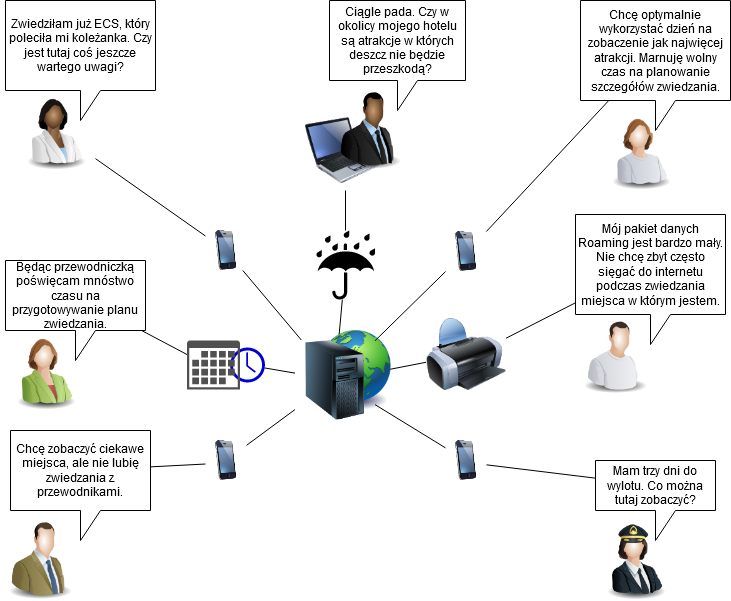
\includegraphics[width=1\textwidth]{attachments/rich-picture}
    \caption{Wzbogacony wizerunek planeru miejskiego}
    \label{fig:rich-picture}
\end{figure}

\section{Cele projektu}
\label{sec:cele-projektu}

TODO

%! Author = Mateusz Budzisz
%! Date = 04/11/2023

\chapter{Decyzje projektowe}
\label{ch:decyzje-projektowe}

\section{Narzędzia i technologie}
\label{sec:narzedzia-i-technologie}

\subsection{Języki programowania i biblioteki}
\label{subsec:jezyki-programowania-i-biblioteki}

\subsubsection{Oprogramowanie po stronie użytkownika}
Jednym z celi projektu jest stworzenie aplikacji progresywnej dostępnej na większości urządzeń codziennego użytku tj.: komputery i smartfony.
Według statystyk prowadzonych przez Google za znaczną część konsumenckiego ruchu internetowego odpowiadają te systemy operacyjne: Android, ios, MacOS, Windows, Linux.
To aż 5 bardzo różniących się od siebie środowisk docelowych, każde z nich posiada swój dedykowany sposób wytwarzania i utrzymywania oprogramowania.
Nasz zespół składający się z czterech pracujących na etacie studentów nie byłby w stanie stworzyć a co dopiero utrzymywać rozwiązania na tylu różnych platformach na raz.
Istnieją rozwiązania niwelujące ten problem w znacznym stopniu, zespół projektowy przeanalizował część z nich pod kątem naszego doświadczenia.

\paragraph{Flutter}
Jest otwartoźródłowy zestaw narzędzi dla programistów przeznaczony do tworzenia natywnych, wieloplatformowych aplikacji mobilnych, komputerowych oraz internetowych, stworzony przez firmę Google.
Aplikacja stworzona w tej technologii pozwala na napisanie kodu źródłowego w jednej wersji i uruchomienie go na szerokiej gamie zróżnicowanych urządzeń docelowych.
Problemem tej technologii jest dość niszowy język programowania, z którym nikt z nas nie miał do czynienia oraz relatywnie słaba wydajność dostarczonego oprogramowania.

\paragraph{Electron}
Jest to otwartoźródłowy projekt, który umożliwia stworzenie oprogramowania w formie strony internetowej oraz osadzenia jej w minimalistycznej wersji przeglądarki wysyłanej wraz z aplikacją.
Dużym plusem tej technologii jest to, że na uczelni mieliśmy zajęcia z React-a, który jest jedną z opcji pisania aplikacji w Electron-ie.
Minusem tego rozwiązania jest bardzo duży rozmiar docelowej aplikacji z uwagi na potrzebę doczepienia przeglądarki internetowej poza samą aplikacją.

\paragraph{Progresywna Aplikacja Internetowa}
Z języka angielskiego Progressive Web App to aplikacja internetowa uruchamiana tak jak zwykła strona internetowa, ale umożliwiająca stworzenie wrażenia działania jak natywna aplikacja mobilna lub aplikacja desktopowa.
Technologia bardzo podobna do Electron-a, z tym że zamiast wysyłać spreparowaną przeglądarkę, polegamy na przeglądarce uprzednio zainstalowanej u użytkownika.
Plusem jest bardzo mały rozmiar docelowej aplikacji oraz relatywnie dobra wydajność, ponieważ przeglądarki internetowe są specjalnie optymalizowane pod wiele platform docelowych.
Minusem tego rozwiązania jest poleganie na przeglądarce użytkownika docelowego, która może nie wspierać wszystkich funkcjonalności.

\paragraph{Wybór}
Każda z wymienionych opcji ma swoje poważne wady.
Nasz zespół podejmując dedycję, kierował się następującymi priorytetami: znajomość technologii wewnątrz zespołu, wydajność rozwiązania.
Biorąc pod uwagę te 2 czynniki, postawiliśmy na \acrshort{pwa}\@.
Pragnąc wykorzystać komercyjne doświadczenie zespołu, zamiast używać poznanego na uczelni React-a, zaimplementujemy aplikację we framework-u Angular.

\subsubsection{Oprogramowanie niewidoczne dla użytkownika}
Nasz projekt zakłada stworzenie zaawansowanego algorytmu ustalania optymalnej trasy zwiedzania na podstawie danych czasu rzeczywistego.
Ciągłe aktualizacje danych po stronie użytkowników spowodowałoby wysokie zużycie internetu oraz ogromne obciążenie po stronie dostawców danych.
Dlatego postanowiliśmy stworzyć serwis, który będzie odpowiadać za aktualność danych oraz wyznaczanie trasy.
Z uwagi na \acrshort{pwa}, język, w którym stworzymy ten serwis, musi mieć bardzo dobre wsparcie dla protokołu HTTP\@.
Na uczelni poznaliśmy 2 technologie tworzenia takich serwisów.

\paragraph{Java}
Java to język paradygmatu obiektowego, bardzo popularny w systemach bankowych.
W trakcie zajęć na uczelni poznaliśmy sposób tworzenia serwisów \acrshort{http} w technologii Spring.
Części naszego zespołu nie podobają się konwencje narzucone przez tę technologię, jak i sposób komunikacji z bazą danych.
Należy zaznaczyć, że nikt z naszego zespołu nie posada komercyjnego doświadczenia z tą technologią.

\paragraph{.NET}
C\# to jeden z języków z rodziny .NET, który mielimy szanse poznać na uczelni.
Łączy on w sobie paradygmaty obiektowe i funkcyjne, dzięki czemu jest bardziej elastyczny, jeśli chodzi o styl programowania.
Trzy z czterech osób w naszym zespole ma doświadczenie komercyjne w tej technologi.

\paragraph{Wybór}
Z uwagi na doświadczenie zespołu postawiliśmy na C\#.

\subsubsection{Baza danych}
Na uczelni dogłębnie poznaliśmy bazę danych PostgreSql, zespół ma komercyjne doświadczenie z tą bazą, więc nie braliśmy innych rozwiązań pod uwagę.

\subsection{Narzędzia programistyczne}
\label{subsec:narzedzia-programistyczne}
Nasz zespół składa się z osób, które mają znaczne doświadczenie w oprogramowaniu, którego używa na co dzień w pracy.
Wybrany przez nas stos technologiczny składa się z .NET C\#, Angular oraz PostgreSql.
Wszystkie te technologie, pomimo iż są utrzymywane przez ogromne korporacje, są otwarto-źródłowe, co w praktyce pozwala na tworzenie narzędzi deweloperskich przez niezależnych twórców, dzięki czemu nie bylibyśmy uwiązani do konkretnego rozwiązania.
Wybór oprogramowania do tworzenia kodu został podyktowany wybraną technologią a w drugiej kolejności z uwagi na zróżnicowany sprzęt komputerowy, którym dysponujemy  dostępnością oprogramowania na wielu platformach (tj.: Windows, MacOS, Linux).

\subsubsection{.NET/C\#}
.NET to framework stworzony i rozwijany przez Microsoft wspólnie ze społecznością otwartego oprogramowania.
Pierwszym oprogramowaniem, które przychodzi nam do głowy, gdy słyszymy .NET, jest Microsoft Visual Studio.
Oprogramowanie to powstało w 1997 roku i przez wiele lat było konsekwentnie ulepszane.
W 2016 roku VS zostało wydane na komputery Mac, jednakże, po 7 latach, w 2023 roku Microsoft ogłosił zakończenie wsparcia dla wersji MacOS.
Jeśli chodzi o systemy Linux, to VS nigdy nie zostało wydane na ten system.

Zespół projektowy bardzo nie chciał uzależnić pracy nad projektem od systemu Windows, Microsoft poleca użycie programu Visual Studio Code, który jest wspierany na wszystkich systemach operacyjnych, których używamy.
Niestety VSC jest edytorem przeznaczenia ogólnego, co za tym idzie, znaczna większość specjalistycznych dla danej technologii narzędzi jest obsługiwana przy pomocy rozszerzeń.
Rozszerzenia mogą tworzyć wszyscy, jest ich całkiem sporo niestety wszystkie rozszerzenia skupiające się na technologii .NET/C\# są we wczesnej fazie rozwoju i nie wspierają tak podstawowych rzeczy, jak debugowanie kodu.
Nawet gdy dane rozszerzenie wspiera jakąś zaawansowaną funkcjonalność, to przeważnie konfiguracja takiego rozszerzenia bardzo różni się pomiędzy systemami operacyjnymi co, de facto niweczy sens wieloplatformowości.

W 2016 roku został ogłoszony JetBrains Rider niejako odpowiedź na VS na MacOS od Microsoftu.
Rider bardzo dynamicznie się rozwijał, nadganiając, a nawet prześcigając VS pod względem funkcjonalności, do momentu, w wyniku czego duża część środowiska programistycznego zaczęła go używać jako głównego narzędzia do pracy.
Programy firmy JetBrains są znane ze świetnej integracji wieloplatformowej oraz dbania o szczegóły, co zapewnia dobre doświadczenie deweloperskie.

Dzięki PJATK nasz zespół mógł przetestować, każdy z tych programów w ramach licencji edukacyjnej.
Nasze testy doprowadziły nas do decyzji, aby postawić na Ridera od JetBrains-ów, z zachowaniem możliwości uruchomienia projektu w Visual Studio, aby koledzy z dużym doświadczeniem komercyjnym opartym o VS nie musieli zmieniać swoich przyzwyczajeń.

\subsubsection{Angular}
Angular z natury bycia technologią tworzenia stron internetowych nie posiada dedykowanego środowiska programistycznego stworzonego przez jedną firmę.
Zespół tworzący ten framework stworzył własny program wspomagania deweloperów na podstawie protokółu \acrshort{lsp}, co sprowadza się do tego, że każde środowisko programistyczne wspierające ten protokół zapewni ten sam poziom wsparcia dla Angular'a.

Warto tu wyróżnić Visual Studio Code, ponieważ jest to środowisko zalecane przez twórców Angular-a, a nowe projekty tworzone w tej technologii zawierają niezbędną konfigurację potrzebną do pełnego wsparcia dla Angulara.

JetBrains też ma w swojej ofercie program do tworzenia w technologiach internetowych o nazwie WebStorm, który posiada automatyczną konfigurację dla Angular-a, jak i wielu innych technologii, więc nie potrzebuje bezpośredniego wsparcia od autorów technologi.

Mając na uwadzę fakt, że Visual Studio Code domyślnie ma skróty klawiszowe nieprzypominające innych popularnych środowisk programistycznych, których trzeba by było się nauczyć, oraz fakt, że już wybrany Rider jest niemalże identyczny w obsłudze do WebStorm'a, postawiliśmy na WebStorm'a, znowu z możliwością uruchomienia projektu w dowolnym innym środowisku, gdy ktoś będzie tego z jakiegoś powodu potrzebował.

\subsubsection{PostgreSql}
W przypadku baz danych przeważnie jest tak, że twórcy bazy danych, równocześnie do samej bazy danych rozwijają narzędzie pozwalające na administrację tą bazą.
W przypadku PostgreSql narzędzie to nazywa się pgAdmin, umożliwia kompleksową konfigurację bazy danych i administrowanie nią.

Należy jednak wspomnieć tu o integracji Ridera z bazą danych we współpracy z programem DataGrip.
Gdy mamy licencję na DataGrip-a, to wewnątrz Rider-a możemy podłączyć się do bazy danych i otrzymywać dodatkowe wsparcie w kontekście bazy danych.
Wsparcie nie ogranicza się tylko do dodatkowego kolorowania składni w zależności od dialektu wybranej bazy danych, a deweloper jest wspierany przez podpowiadanie nazw kolumn, tabeli oraz poprawność zapytań do bazy jest  weryfikowana w czasie rzeczywistym, a w przypadku wątpliwości Rider pozwala na szczegółową analizę kwerendy w DataGrip'e.

Mając na uwadze powyższe, zespół projektowy zaleca użycie DataGrip-a jako narzędzia do projektowania rozwiązań dookoła bazy danych z uwagi na kompleksową integrację z Riderem.

\subsubsection{Dalekosiężność wyborów}
W przypadku, w którym zespół zdecydowałby się na dalsze utrzymywanie bądź rozwój projektu, należy brać pod uwagę koszta oprogramowania.

Visual Studio jest najdroższym z wymienionych rozwiązań, do tego wspiera tylko wąski fragment stosu technologicznego.

Oprogramowanie JetBrains, na które postawiliśmy, jest dostępne jako poszczególne programy w formie abonamentu, jednakże najkorzystniej jest je kupować w pakietach łączonych.

Warto też wspomnieć o programie wsparcia open source firmy JetBrains, która to oferuje darmowe licencje do wszystkich swoich komercyjnych rozwiązań dla projektów o otwartym kodzie źródłowym, przy czym nasz projekt spełnia tę definicję.

Ponadto dzięki zachowaniu kompatybilności z alternatywnymi środowiskami deweloperskimi, jesteśmy w stanie małym nakładem pracy zmienić oprogramowanie nawet na darmowe.

\subsection{Dostawcy mocy obliczeniowej}
\label{subsec:dostawcy-mocy-obliczeniowej}
Wytworzone oprogramowanie potrzebuje serwerów, na których będzie wdrożone.
Zespół projektowy zna 2 podejścia do tego problemu.

\subsubsection{Oprogramowanie w chmurze}
Dostawcy oprogramowania w chmurze umożliwiają bardzo elastyczny system rozliczania się za moc obliczeniową.

Gdy aplikacja nie wymaga ciągłej pracy oraz w sposób deterministyczny można ustalić warunki czasowe dla aplikacji, możemy jej użyć w stylu \gls{on-demand}.
Sposób ten charakteryzuje bardzo korzystny sposób rozliczania, gdzie płacimy za faktycznie wykorzystany czas pracy maszyn oraz potencjalnie nieskończone możliwości horizontal-scallingu.

Wybór takiego rozwiązania mocno wpłynąłby na architekturę naszego rozwiązania.
Niejako wymusiłby na nas, podział projektu na niezależne od siebie moduły i z uwagi na bardzo skomplikowany \gls{refactoring} przy 4-osobowym zespole de facto scementowałby strukturę projektu.

Nasz projekt teoretycznie można podzielić na niezależne od siebie części o różnym zapotrzebowaniu na moc obliczeniową.
Pierwszym modułem musi być baza danych, w której będziemy trzymać graf możliwych połączeń między atrakcjami oraz informacje o samych atrakcjach, ten moduł musiałby być cały czas dostępny z uwagi na duży koszt wyprodukowania danych, przeważający koszt utrzymania bazy w sposób ciągły.
Drugim modułem mógłby być \gls{job} aktualizujący dane z OSM, urzędu miasta oraz atrakcji turystycznych, taki moduł mógłby uruchamiać się na przykład raz dziennie.
Trzecim modułem byłby serwis implementujący algorytm, dobierania trasy pomiędzy podanymi POI, taki serwis uruchamiałby się na zapytanie użytkownika i kończył swoją pracę wraz z podaniem optymalnie dobranej trasy.
Ostatnim modułem byłaby aplikacja \gls{frontend}-owa implementująca UI, włączana z osobna dla każdego użytkownika, gdy ten podejmie próbę wejścia na adres naszego rozwiązania.

Takie podejście w praktyce zmniejsza koszt utrzymania do kosztu utrzymywania bazy danych, ponieważ gdy zapotrzebowanie na pozostałe moduły drastycznie by zmalało, to nie będą one chodzić i czekać na ruch użytkowników.
Niestety uruchamianie programów na żądanie wiąże się ze znaczącym opóźnieniem wobec żądań użytkownika docelowego.
Gdy użytkownik postanowi skorzystać z naszej aplikacji, dostawca chmury obliczeniowej musi uruchomić co najmniej dwie maszyny, dla modułu 3 i 4, co czasami potrafi zająć kilka sekund.
Gdy dostawca chmury uruchomi odpowiednie maszyny, jeszcze nasze oprogramowanie wymaga czasu na obsłużenie żądania.
W przypadku modułu 3 musimy nawiązać połączenie z bazą danych, odczytać dane, zastosować na nich skomplikowany obliczeniowo algorytm i wysłać odpowiedź, obawiamy się, że w skrajnych przypadkach może to zająć za dużo czasu aby odpowiedź trafiła do użytkownika przed zamknięciem połączenia.
W przypadku modułu 4 możemy odroczyć oczekiwanie na odpowiedź modułu 3 i poinformować użytkownika o wydłużonym czasie oczekiwania, niemniej jednak, aby cokolwiek użytkownikowi pokazać i tak jesteśmy zmuszeni do wykonania kodu odpowiedzialnego za stworzenie \gls{ui}, według doświadczeń zespołu czas potrzebny na \gls{rendering} \gls{hello-world} pozostawia niewiele czasu do przekroczenia średniego time span nowego użytkownika (TODO: source).

Istnieją techniki pozwalające na optymalizację tych rozwiązań, aby wyeliminować przytoczone problemy.
Jednak opierają się one o jeszcze większą fragmentację aplikacji, na którą nie możemy sobie pozwolić z uwagi na liniowo rosnący czas potrzebny na konfigurację infrastruktury potrzebnej do skomunikowana wszystkich modułów w \glslink{hermetyzacja}{hermetyczny} sposób.
Infrastrukturę chmury internetowej w każdym ze znanych nam dostawców to jest: \acrshort{aws}, \acrshort{gcp}, \acrshort{azure} możemy wyklikać w przeglądarce internetowej.
Jednak usługi te znacząco się od siebie różnią.
Możemy tę manualną pracę zautomatyzować przy pomocy podejścia \gls{infra-as-code}, na przykład przy użyciu terraform.
Pomimo iż dostawcy oferują podobne rozwiązania, to różnią się one w sposobie konfiguracji, na przykład 1 usługa w \acrshort{gcp} to 3 usługi w \acrshort{aws}\@.
Terraform daje możliwość skorzystania z dodatkowej warstwy abstrakcji pozwalającej na opisanie architektury dla \acrshort{aws}, jak i zarówno \acrshort{gcp}, jednakże nie jest to pełne wsparcie i niektóre usługi po prostu nie pokrywają się pomiędzy dostawcami.
Ponadto Terraform nie wspiera takiej funkcjonalności dla Azure.

\subsubsection{Oprogramowanie on premise}
Oprogramowanie on premise możemy podzielić na bare metal i virtual.

Bare metal to takie, gdzie mamy fizyczny dostęp do maszyny i płacimy za konkretne podzespoły, mamy pełną kontrolę nad maszyną.
Virtual to oprogramowanie, w którym tak jak w przypadku bare-metal musimy sami zarządzać maszyną.
Różni się jednak tym, że płacimy za parametry podzespołów, nie za konkretne podzespoły.
Nie mamy też fizycznego dostępu do maszyny, ponieważ parametry, jakich potrzebujemy, mogą być mniej wymagające, niż fizyczna maszyna jest w stanie zapewnić, przez to właściciele takich maszyn stosują \glslink{virt}{wirtualizację}.

Bare metal ma taką zaletę, że jesteśmy pewni, że nikt poza nami na takiej maszynie nie będzie pracował.
Minusem jest mała elastyczność podzespołów (musimy wiedzieć, co będzie działać, z czym) oraz wysoki koszt początkowy.
W przypadku wirtualizacji na początku rozwoju aplikacji możemy poprosić o niewielkie parametry a wraz z rozwojem przeskalować parametry do naszych potrzeb.

Pomimo faktu, iż w przypadku \gls{on-prem} musimy sami zarządzać infrastrukturą, to jest to niezależne od dostawcy sprzętu, dzięki czemu można łatwo przenieść całą aplikację do innego dostawcy.
Biorąć pod uwagę ten fakt oraz brak możliwości napisania oprogramowania w sposób pełni agnostyczny względem konkretnych usług chmury obliczeniowej, zespół projektowy zdecydował się na on premise w wariancie virtual.

\subsubsection{Przegląd rynku}
\paragraph{Microsoft Azure Cloud}
Chmura obliczeniowa Microsoftu została nam udostępniona w ramach zajęć z konteneryzacji.
Microsoft udostępnia studentom jednorazowo 200\$ do wykorzystania na okres roku.
W ramach okresu edukacyjnego mamy do dyspozycji najsłabsze i najmniej stabilne maszyny dostępne w ofercie.
W trakcie zajęć natknęliśmy się na wiele problemów ze stabilnością i wydajnością tej chmury.
Jednorazowy roczny okres próbny w połączeniu z ograniczeniem budżetowym całkowicie deklasuje tą chmurę z powodu braku możliwości utrzymania rozwiązania w rozumieniu długoterminowym

\paragraph{Amazon Web Services}
Chmurę obliczeniową Amazon mieliśmy okazję zobaczyć na szkoleniu organizowanym przez Merapar.
W trakcie zajęć chmura nie sprawiła najmniejszych problemów, co pokrywa się z licznymi opiniami rynkowymi.
Niestety pomimo wielu darmowych progów zużycia, Amazon nie oferuje darmowego progu w przypadku usługi EC2 (\gls{on-prem} virtual).

\paragraph{Google Cloud Platform}
GCP zostało nam zaprezentowane w ramach projektu PJATK cloudelina.
Usługi w ramach GCP wydają się znacznie prostsze w konfiguracji oraz bardzo dobrze integrują się z Angular-em.
Niestety podobnie jak w przypadku Amazon-u, GCP nie oferuje darmowego progu dla maszyn wirtualnych.

\paragraph{Oracle Cloud Platform}
Oracle cloud jako jedyne nie posiada usług typowych dla architektury chmurowych.
Oracle daje bardzo hojny darmowy limit dla maszyn wirtualnych opartych o \glslink{arm}{architekturę arm} wynoszący 6 CPU, 24 GB RAM, 200 HDD i 100 Mbs ethernet.
Taki próg pozwoli nie tylko na wytworzenie oprogramowania, przeprowadzenie testów, ale nawet i obsługę średniej wielkości ruchu użytkowników.

\subsection{Przechowywanie kodu oraz potok ciągłego wdrożenia}
\label{subsec:przechowywanie-kodu-oraz-potok-ciagego-wdrozenia}

W trakcie zajęć na uczelni, jak i pracy indywidualnej członków zespołu projektowego poznaliśmy 2 systemy kontroli wersji.
Są to GIT oraz Mercurial.

GIT pod każdym względem jest lepszy od Mercurial, sam Mercurial jest uznany za projekt bez rozwoju.
Zespół projektowy postanowił oprzeć swoją pracę na podstawie GIT, natomiast nie chcemy samodzielnie zarządzać serwerem repozytorium.

\subsubsection{Usługi internetowe ułatwiające pracę wielu współbieżną w repozytorium GIT}
\paragraph{GitLab}
\paragraph{BitBucket}
\paragraph{Microsoft Azure Repositories}
\paragraph{Github}



	%! Author = Wiktor Rostkowski
%! Date = 29/04/2024

\chapter{Analiza Rynku}
\label{ch:analizy-rynku}

%! Author = Wiktor Rostkowski
%! Date = 05/1/2024


\section{Aspekty Społeczne}
\label{subsec:aspekty-spoleczne}



 \indent Niestety, w erze „fake news”, gdzie występuje duża ilość niskiej jakości informacji, trudno znaleźć potrzebne nam kompendium wiedzy. Każda grupa społeczna, od młodzieży do seniorów, jest podatna na tę sytuację[].
Aplikacja odpowiada na wiele potrzeb turystów, którzy chcą poruszać się po nieznanym mieście. Jest swoistym zbiorem wiedzy potrzebnej dla każdego turysty, bez żadnych niedopowiedzeń. Dlatego przewidywaną grupą docelową są osoby odwiedzające daną miejscowość z umiarkowaną znajomością technologii, personalizujące podróż dla siebie lub dla większej grupy osób, na przykład wycieczki dla znajomych.



\indent Na potrzeby turystów proponujemy rozwiązanie z poniższymi funkcjami:

\begin{enumerate}
   \item 	Generowanie planu wycieczki na podstawie wybranych zainteresowanych nas miejsc drogę pomiędzy nimi
   \item 	Automatyczna aktualizacja planu zwiedzania na podstawie dynamicznych wydarzeń, takich jak zmiana pogody, rozkład jazdy czy dostępność atrakcji, co umożliwia planowanie w czasie rzeczywistym.
   \item	Interaktywna mapa z naniesionymi atrakcjami turystycznymi zawierająca zawsze aktualne informacje o atrakcjach turystycznych
\end{enumerate}

\indent Dzięki takim funkcjonalnościom można uniknąć wielogodzinnego poszukiwania odpowiednich informacji na temat dostępnych miejsc jak i zaplanować podróż.

\paragraph*{Społeczne aspekty}\\
\indent Przeprowadzona została analiza społecznych aspektów realizowanego projektu, na podstawie której wyodrębnione zostały zarówno pozytywne, jak i negatywne skutki.  Poniżej zaprezentowane zostały wyniki analizy.\\

\indent Jednym z założeń projektu jest promowanie rozwoju turystyki. Aplikacja pozwala na promowanie niszowych atrakcji.\\
Z tego powodu przedstawiamy na mapie tylko atrakcje turystyczne, znaczników jest mniej, więc mniej popularne atrakcje mają większą szansę na odnalezienie przez użytkownika.

\indent Przedstawione informacje są jak dostępne dla każdego odwiedzającego, przez znormalizowane źródło informacji potrzebne turystom nie tylko informacje o atrakcjach, ale też dostępny transport a w przyszłości  możliwe zakwaterowanie oraz restauracje.
Dzięki temu każda osoba ma mniejszy próg wejścia w podróżowania i może zrezygnować z potrzeby posiadania przewodnika.
Takie informacje przekładają się na oszczędność czasu dla każdego podróżnika, chcącego korzystać z przyjemności zwiedzenia a nie szukania informacji w Internecie czy przeglądając fora podróżnicze lub papierowe przewodniki.


\indent Ponadto, eliminacja obracania się danymi wrażliwymi w przyjętym modelu przyczynia się do zwiększenia poczucia bezpieczeństwa użytkowników. Korzystanie z systemu nie niesie dla nich ryzyka utraty lub nieuprawnionego wykorzystania danych, co jest istotne dla zachowania zaufania. Misją zespołu projektowego jest zaspokajanie potrzeb użytkowników z uwzględnieniem ich interesów oraz przestrzeganie obowiązującego prawa, przy jednoczesnym unikaniu wszelkich form dyskryminacji.
W związku z powyższym zarysowują się obszary, w których można ulepszyć, wyłaniają się obszary, w których można przyszłościowo ulepszyć proponowany system tak, aby lepiej zaspokajał potrzeby użytkowników oraz miał większy wpływ społeczno-etyczny. Istotnym krokiem byłoby umożliwienie użytkownikowi dostosowania kolorystyki i czcionek w aplikacji, co jest szczególnie istotne dla osób z zaburzeniami widzenia, trudnościami w rozpoznawaniu barw.

\paragraph*{Negatywne czynniki społeczne:}

\indent Po pierwsze, wytworzona aplikacja umożliwia użytkownikom samodzielny i łatwy dostęp do informacji obecnie trudno dostępnych, zatem w konsekwencji może zwiększać poczucie zagrożenia u przewodników turystycznych funkcjonujących na wolnym rynku. \newline

\indent Po drugie, istnieje ryzyko utraty danych związanych z nieukończonym procesem wybierania trasy, szczególnie gdy użytkownik korzysta z aplikacji bez posiadania konta użytkownika. Ponadto, dane takie jak trasy i atrakcje są przechowywane w pamięci przeglądarki, co zwiększa ryzyko ich utraty, jeśli użytkownik nie jest zalogowany. Co więcej, użytkownik może stracić dane podczas zmiany urządzenia bez wcześniejszego zalogowania się na obu z nich.\newline 

\indent Warto także nadmienić, iż od początku projektowania aplikacji nie uwzględniono kilku funkcjonalności, które obecnie mogą generować pewien niedosyt dla użytkownika. Na przykład, brak możliwości rezerwacji terminów w wybranych atrakcjach może stanowić problem dla niektórych użytkowników, szczególnie, gdy wymaga to wcześniejszej rezerwacji. Ponadto, użytkownik musi samodzielnie zaplanować przerwy, co może być kłopotliwe dla niektórych osób. Brak integracji z zakwaterowaniem w początkowej fazie rozwoju aplikacji może również ograniczać możliwości użytkowników w planowaniu podróży.\newline

\indent Dyskryminacja użytkowników w kontekście integracji komunikacji miejskiej w danej miejscowości z naszą aplikacją może wynikać z różnic w jakości danych oraz dostępności funkcji dla użytkowników w zależności od miejsca ich pobytu.
Jeśli miasto nie zdecyduje się na pełną integrację z naszą aplikacją, dane związane z tym obszarem mogą być mniej kompleksowe i aktualne niż w przypadku miast, które aktywnie uczestniczą w projekcie. W rezultacie użytkownicy korzystający z naszej aplikacji w takich obszarach mogą napotkać na braki informacji, błędne dane czy ograniczone możliwości korzystania z funkcji.

\paragraph{Paragraf}



%! Author = Wiktor Rostkowski
%! Date = 05/1/2024


\section{Aspekty Biznesowe}
\label{sec:aspekty-biznesowe}



Jakiś wstęp

\paragraph{Paragraf}



%! Author = Wiktor Rostkowski
%! Date = 05/1/2024


\section{Analiza Ryzyka}
\label{subsec:analiza-ryzyka}

\pagebreak
\begin{longtable}{|p{.1\linewidth}|p{.15\textwidth}|p{.2\textwidth}|p{.25\textwidth}|p{.25\textwidth}|}
    \hline
    Ryzyko & Czynniki ryzyka & Charakterystyka ryzyka & Prawdopodobieństwo wystąpienia ryzyka & Planowane działania \\
    \hline
    \multirow{6}{=}{\parbox[c]{11cm}{\rotatebox{90}{\textbf{Nieukończenie projektu w terminie}}}}& Rozpad grupy & Odejście jednego z członków zespołu & niskie 
    & Przejrzysta komunikacja w zespole i ustalenie wersji MVP produktu, która może zostać ukończona w uszczuplonym składzie \\
    \cline{2-5}
     & Czasowa niedostępność/niedyspozycja członka zespołu & Nagła lub zaplanowana nieobecność członka zespołu & średnie 
     & Możliwie wczesne sygnalizowanie planowanej nieobecności \\
     \cline{2-5}
     & Zbyt ambitne założenia projektowe & Zaplanowane prace wykraczają poza moce przerobowe członków zespołu & średnie
    & Śledzenie postępu prac pod kątem wykonalności i zmieszczenia się w ograniczeniach czasowych, konsultacja z promotorem \\
    \cline{2-5}
     & Pełzające wymagania & Ciągle powiększana pula wymagań, zwiększająca zakres prac do wykonania & średnie & \\
     \cline{2-5}
     & Nauka nowych technologii/języków programowania & Zwiększenie ilości czasu potrzebnej na ukończenie zadania & 
     wysokie & \\
     \cline{2-5}
     & Problem z komunikacją w zespole & Brak właściwego przepływu informacji między członkami zespołu & średnie
     & Cykliczne spotkania członków zespołu w celu omawiania postępu prac i planowania kolejnych działań \\
    \hline
    \multirow{5}{=}{\parbox[c]{10cm}{\rotatebox[origin=c]{90}{\multirow{5}{=}{\textbf{Produkt nie spełnia wymagań projektowych}}}}} & Błędna analiza rynku & Niewłaściwe rozpoznanie potrzeb potencjalnych użytkowników oraz rozwiązań konkurencyjnych & niskie
     & Konsultacje z promotorem, stworzenie profilu docelowego użytkownika \\
     \cline{2-5}
     & Niespełnienie wymagań klientów & Finalny produkt nie zapewnia zakładanych korzyści dla użytkownika końcowego & średnie
     & Konsultacje z promotorem, cykliczna analiza kierunku rozwoju produktu \\
     \cline{2-5}
     & Wydanie wersji zawierającej krytyczne błędy & Produkt zawiera błędy uniemożliwiające korzystanie z jego podstawowych funkcjonalności & niskie
     & Napisanie odpowiednich testów sprawdzających działanie funkcjonalności \\
     \cline{2-5}
     & Zmiany w usługach zależnych & Wyłączenie lub zmiana warunków na jakich udostępniane są API wpływa na dostarczane funkcjonalności & średnie
     & Ustalenie alternatywnych dostawców potrzebnych usług \\
     \cline{2-5}
     & Zły dobór narzędzi projektowych & Wybrane narzędzia są nieodpowiednie do zaplanowanych prac & niskie
     & Zaznajomienie się z dokumentacją używanych narzędzi, konsultacje w zespole \\
    \hline
    \multirow{2}{=}{\parbox[c]{3.5cm}{\rotatebox[origin=c]{90}{\multirow{2}{=}{\textbf{Niewłaściwe zaplanowanie przebiegu prac}}}}} & Przyjęcie niedpowiedniej strategii projektowej & Przyjęta strategia nie pozwala na uzyskanie wymaganych rezultatów przy dostępnych zasobach & wysokie
     & Stałe monitorowanie kierunku prac, konsultacje z promotorem \\
     \cline{2-5}
     & Nierozpatrzenie potencjalnych przypadków brzegowych & Konieczność uwzględnienia nieprzewidzianych prac & wysokie
     & Staranne analizowanie planowanych funkcjonalności i ich wpływu na produkt \\
     \hline
     \multirow{1}{=}{\parbox[c]{2cm}{\rotatebox[origin=c]{90}{\multirow{1}{=}{\textbf{Zdarzenia nieprzewidziane}}}}}& Zbyt gwałtowny rozrost liczby użytkowników & Liczba użytkowników przekracza zaplanowane możliwości techniczne produktu & niskie
     & Projektowanie produktu z możliwością jego skalowania \\
    \hline

\end{longtable}
\pagebreak



\chapter{Analiza Rynku}
\label{ch:analiza-rynku}

\section{Rozwiązania konkurencyjne}
\label{ch:rozwiązania-konkurencyjne}

\paragraph{Wstęp}

Na rynku dostępne są obecnie różne rozwiązania mające na celu ułatwienie planowania podróży i posiadające różny zakres funkcjonalności. 
Użytkownik może napotkać rozbudowane aplikacje integrujące wiele funkcjonalności takich jak układanie list atrakcji do zwiedzania,
optymalizacja tras podróży, dokumentowanie poniesionych wydatków, tworzenie list ułatwiających planowanie (listy czynności do wykonania,
listy zakupów, listy ułatwiające organizację pakowania), synchronizacja naszych planów podróży ze znajomymi, integrowanie rezerwacji hotelowych i lotów.
Aplikacje skupiające się na wspomaganiu procesu zwiedzania sugerują użytkownikowi interesujące punkty w jego lokalizacji (interesujące miejsca, hotele,
restauracje, sklepy itp.) i oznaczają je na mapie. Dodatkowo bardzo często są wyposażone w rozbudowany opis danej atrakcji, czasem również w formie
głosowej, co umożliwia zamienienie urządzenia mobilnego w osobisty audio przewodnik. Kolejną funkcjonalność stanowi możliwość dokonywania zakupu biletów
i rezerwowania atrakcji bezpośrednio z poziomu aplikacji turystycznej .Poniżej przedstawiono przykłady najpopularniejszych obecnie rozwiązań 
ułatwiających planowanie zwiedzania.

\paragraph{Wanderlog}

Jest to aplikacja reklamująca się jako planer podróży, ze szczególnym naciskiem na organizowanie wakacji oraz wycieczek samochodem.
W wersji podstawowej jest darmowa, posiada również płatną wersję premium  oferującą dodatkowe funkcjonalności.
Aplikacja jest dostępna poprzez przeglądarkę internetową jak również poprzez dedykowaną aplikację na urządzenia mobilne. 
Wanderlog umożliwia układanie list z interesującymi użytkownika miejscami i wydarzeniami, które są graficznie przedstawione w
postaci pinezek na mapie google. Po wybraniu lokalizacji i daty podróży, użytkownik może dokonać przeglądu ofert noclegów. 
Aplikacja umożliwia tworzenie planów podróży razem z innymi użytkownikami oraz ich synchronizację w czasie rzeczywistym. 
Ponadto użytkownik ma dostęp do spersonalizowanych sugestii.

\paragraph{TripIt}

Jest to planer podróży integrujący wiele funkcjonalności w celu maksymalnego ułatwienia użytkownikowi procesu podróżowania. 
Stanowi alternatywę dla wspomnianej wcześniej aplikacji Wanderlog i również posiada darmową wersję podstawową oraz wersję płatną 
opartą na modelu subskrypcyjnym, która posiada dodatkowe funkcjonalności. W wersji podstawowej użytkownik ma możliwość układania 
planów podróży, które są dostępne na wielu urządzeniach jednocześnie. Udostępnia statystyki, wytyczne dotyczące restrykcji COVID-19
oraz umożliwia dodawanie zdjęć, kodów QR oraz plików PDF do planów podróży. Aplikacja zapewnia nawigację między punktami,
mapy lotnisk, sugestie co do intersujących miejsc blisko lokalizacji użytkownika,
jak również informowania o poziomie niebezpieczeństwa danej okolicy. 
Podstawowa wersja aplikacji umożliwia również dzielenie się planami z innymi użytkownikami oraz synchronizację kalendarza. 
W wersji płatnej użytkownik ma dostęp do szeregu funkcjonalności ułatwiających podróżowanie samolotem, np. informacja o dostępności
lepszych miejsc, przypomnienia o zarezerwowanych lotach, powiadomienia o statusie lotów w czasie rzeczywistym, mapy lotnisk wraz
ze szczegółowymi informacjami o położeniu obiektów, informacje o punkcie odbioru bagażu.

\paragraph{Harmony}

Umożliwia tworzenie planów podróży wraz ze znajomymi w czasie rzeczywistym oraz synchronizację z kalendarzem Google.
Ponadto aplikacja umożliwia śledzenie poniesionych wydatków i podziału kosztów na poszczególne osoby. 
Użytkownik ma możliwość otrzymywania sugestii generowanych przez AI dotyczących interesujących miejsc w danej lokalizacji 
jak również rezerwowania wycieczek w aplikacji. Aplikacja umożliwia również tworzenie list rzeczy do wykonania w
celu łatwego śledzenia postępów. Obiekty do zwiedzania są zwizualizowane na mapie Google w postaci pinezek.

\paragraph{Rove.me}

Jest to aplikacja, która sugeruje użytkownikowi najlepszy czas na odwiedzenie danego miejsca lub wydarzenia w ciągu roku. 
Aplikacja informuje również o typowej pogodzie występującej w interesującym użytkownika miejscu z uwzględnieniem pory roku lub daty.

\paragraph{Roadtrippers}

Umożliwia tworzenie planów podróży ze szczególnym uwzględnieniem podróży samochodem. 
Użytkownik oznacza na mapie interesujące go miejsca takie jak atrakcje, hotele, stacje paliw, sklepy itp. 
i udostępnia informacje o odległości od danej destynacji oraz szacowany czas dotarcia do niej. 
Aplikacja skierowana jest do użytku na terenie Stanów Zjednoczonych.

\paragraph{Visit a City}

Użytkownik ma możliwość tworzenia list obiektów do zwiedzania jak również rezerwowania wycieczek i aktywności w oparciu o dużą bazę dostępnych lokalizacji.
Posiadają one rozbudowane informacje i oceny dodawane przez innych użytkowników, na podstawie których możliwe jest dokonywanie wyborów, ponadto aplikacja
sugeruje interesujące miejsca w pobliżu lokalizacji użytkownika. Aplikacja jest dostępna mobilnie na urządzeniach z systemem iOS i Android.

\paragraph{SmartGuide}

Zamysłem aplikacji jest dostarczenie użytkownikom platformy dzięki której urządzenie osobiste może zostać zamienione w przewodnik turystyczny.
Zwiedzanie odbywa się po zaplanowanych trasach, a dzięki śledzeniu lokalizacji użytkownika za pomocą nawigacji GPS, aplikacja może określić kiedy
osoba zwiedzająca dotarła do interesującego punktu i odtworzyć zapis audio z opisem obiektu. Informacje o oglądanym obiekcie dostępne są również 
w formie tekstowej. Aplikacja skierowana jest nie tylko do turystów, ale również do organizatorów wycieczek, którzy mogą tworzyć własne trasy zwiedzania.

\paragraph{Fodor's City Guide}

Aplikacja rekomenduje użytkownikowi najciekawsze miejsca do zwiedzania oraz najlepsze restauracje, hotele i sklepy, jak również umożliwia rezerwację
tych usług.jest dostępna jest na urządzeniach z systemem iOS.

\paragraph{Tripadvisor}

Aplikacja umożliwia planowanie wycieczek, rezerwację usług  w oparciu między innymi o rekomendacje, opinie oraz wskazówki innych użytkowników.
Rekomendowane miejsca znajdujące się w pobliżu lokalizacji użytkownika są przedstawione na mapie w formie pinezek. Aplikacja umożliwia również dostęp
do zakupionych biletów w formie elektronicznej. Jest dostępna na urządzeniach z systemem iOS i Android.

\paragraph{Podsumowanie}

Wymienione aplikacje różnią się poziomem rozbudowania i co za tym idzie oferowanymi funkcjonalnościami. 
Wspólnym mianownikiem jest możliwość tworzenia list z obiektami do odwiedzenia. Najbardziej rozbudowane aplikacje umożliwiają rezerwowanie usług
oraz środków transportu, a także ustalanie optymalnych tras podróży. Każda z aplikacji oferuje graficzne oznaczenie obiektów na mapie. Aplikacje
pełniące rolę przewodników wyposażone są w informacje turystyczne na temat obiektów odwiedzanych przez użytkownika, czasami również w formie audio.
Użytkownik może również kierować się opiniami i wskazówkami innych zwiedzających, które zostały przez nich zamieszczone na temat danego obiektu,
czy usługi. Na ten moment wydaje się jednak, że żadna z aplikacji nie dysponuje możliwością dynamicznego i zautomatyzowanego układania planu zwiedzania,
który jest dostosowany do zainteresowań i możliwości czasowych użytkownika odwiedzającego dane miejsce.

	%! Author = Wiktor Rostkowski
%! Date = 29/04/2024

\chapter{Planowanie}
\label{ch:planowanie}



\chapter{Analiza wymagań}
\label{ch:analiza_wymagan}

%! Author = Wiktor Rostkowski
%! Date = 29/04/2024




\section{Wymagania ogólne i dziedzinowe }
\label{sec:wymagania-ogolne-i-dziedzinowe}




%! Author = Wiktor Rostkowski
%! Date = 29/04/2024



\section{Wymagania funkcjonalne}
\label{sec:wymagania-funkcjonalne}



%! Author = Wiktor Rostkowski
%! Date = 29/04/2024




\section{Interfejs z otoczeniem }
\label{sec:interfejs-z-otoczeniem}



%! Author = Wiktor Rostkowski
%! Date = 29/04/2024


\section{Wymagania niefunkcjonalne}
\label{sec:wymagania-niefunkcjonalne}


%! Author = Wiktor Rostkowski
%! Date = 29/04/2024




\section{Wymania dotyczące procesu wytwarzania}
\label{sec:wymania-dotyczace-procesu-wytwarzania}


%! Author = Wiktor Rostkowski
%! Date = 29/04/2024




\section{Wymagania jakościowe i inne}
\label{sec:wymagania-jakosciowe-i-inne}




	\include{chapters/Solution-contents-sol}
	%! Author = Wiktor Rostkowski
%! Date = 29/04/2024

\chapter{Metodologia Pracy}
\label{ch:metodologia-pracy}

%! Author = Wiktor Rostkowski
%! Date = 29/04/2024




\section{Środowiska Docelowe}
\label{sec:srodowiska-docelowe}

\section{Ramowy harmonogram zadań i wykres Gantt’}
\label{sec:ramowy-harmonogram-zadan-i-wykres-gantt’}


\section{ System kontroli wersji i współdzielenie dokumentów projektowych}
\label{sec:-system-kontroli-wersji-i-wspoldzielenie-dokumentow-projektowych}



	\include{chapters/Tests-contents-test}
	\include{chapters/Summary-contents-sum}



	% Początek słownika, akronimów i bibliografii
	\printbibliography[heading=bibintoc]
	\printglossary[type=\acronymtype]
	\printglossary
	% Koniec słownika, akronimów i bibliografii

\end{document}
